\documentclass[11pt]{article}

\usepackage[utf8]{inputenc}
\usepackage[T1]{fontenc}
\usepackage[margin=1in]{geometry}
\usepackage{graphicx}
\usepackage{booktabs}
\usepackage{amsmath}
\usepackage{siunitx}
\usepackage{caption}
\usepackage{orcidlink}
\usepackage{hyperref}
\hypersetup{hidelinks}
\usepackage{xcolor}

\captionsetup{font=small,labelfont=bf}
\setlength{\parskip}{4pt}
\setlength{\parindent}{0pt}

\title{\textbf{Prefix-token steering of a SELFIES language model toward a\\
target UV-Vis absorption band under a structural screen}}

\author{Julian M. Kleber\,\orcidlink{0000-0001-5518-0932}\\
\small ORCID: 0000-0001-5518-0932\\
\small Independent researcher, Berlin, Germany}

\date{\today}

\begin{document}
\maketitle

\begin{abstract}
\noindent
A small molecular language model can be steered toward a target optical property by
prepending control tokens to its training sequences, but the size of that effect is
rarely measured against an identical unsteered model at scale. This work trains a
two-layer GRU language model over SELFIES strings on ZINC250k (249{,}455 molecules) in
two arms that share architecture, data and training budget. The steered arm prepends two
prefix control tokens, a target UV-Vis absorption band and a structural-screen flag. The
plain arm receives none. Absorption maxima are scored by a surrogate model, a Morgan
ECFP fingerprint fed to a gradient-boosted regressor trained on a public UV-Vis dataset,
with a held-out mean absolute error of 24.0~nm. Over 20{,}000 samples per arm and a
target band of 400 to 450~nm, prefix steering raises the fraction of molecules predicted
to fall in band from 0.187 to 0.237, a difference of 0.050 with a 95\% bootstrap
confidence interval of [0.043, 0.058] that excludes zero. The structural-screen pass rate
rises from 0.964 to 0.999. Validity stays at 1.000 and uniqueness and novelty stay near
0.999 in both arms. The effect is real and modest. Most samples still fall outside the
band, and the property values are surrogate predictions, not measurements. The
structural rules act only as a pass or fail screen and a conditioning flag. They are
never a generation target and never a reward. Code and the evaluation artifacts are
public.
\end{abstract}

\section{Introduction}

De novo molecular generators are routinely steered toward target properties such as
drug-likeness, lipophilicity or activity against a target. The common recipes are a
property-conditioned language model, reinforcement-learning fine-tuning, or classifier
guidance in a diffusion sampler \cite{blaschke2020reinvent, wang2021mcmg, vignac2023digress}.
A separate line of work enforces hard constraints inside the sampler, so that every
generated sequence satisfies a stated rule by construction
\cite{cardei2025cdd, christopher2025nsd}.

Soft conditioning, the family this paper studies, raises the rate of on-target samples
without any per-sample guarantee. The open practical question is how large that rate
increase is for a concrete optical-property target, measured honestly against an
identical model that receives no conditioning signal, at a sample size large enough to
separate the effect from sampling noise. This paper answers that question for one target,
the first UV-Vis absorption maximum, on one band, with one model and one seed.

The contribution is narrow and empirical:
\begin{itemize}
  \item A controlled two-arm comparison in which the only difference is two prefix
  control tokens, measured over 20{,}000 samples per arm with a bootstrap confidence
  interval on the steering effect.
  \item An honest account of the effect size, its uncertainty, and the limits of a
  surrogate property model whose error (24.0~nm) is about half the width of the target
  band.
\end{itemize}

This is ordinary optical and dye chemistry. The structural rules used here are a
screening metric and a conditioning flag. They are never optimised toward and never used
as a reward. There is no synthesis, no reaction planning and no route prediction anywhere
in this work.

\section{Methods}

\subsection{Data}

The training corpus is ZINC250k, the standard drug-like subset of ZINC
\cite{sterling2015zinc15}, as released in the \texttt{chemical\_vae} distribution,
249{,}455 molecules. Each molecule is encoded as a SELFIES string
\cite{krenn2020selfies}, which guarantees that every decoded string is a
valence-valid molecule, so reported validity reflects RDKit \cite{rdkit} parse success, not raw string syntax.

The property model is trained on a public experimental UV-Vis dataset
\cite{joung2020uvvis}. The raw release holds 20{,}236 records. After removing rows
without a numeric first absorption maximum and canonicalising structures, 6{,}425 unique
structures remain, with absorption maxima from 162 to 878~nm.

\subsection{Surrogate property model}

Each structure is converted to a Morgan ECFP fingerprint (radius 2, 2048 bits) and
passed to a scikit-learn \texttt{HistGradientBoostingRegressor}
\cite{pedregosa2011scikit} that predicts the first absorption maximum in nm. On a random
held-out split (5{,}203 train, 643 test structures) the regressor reaches a mean absolute
error of 24.0~nm, a root-mean-square error of 38.2~nm and a coefficient of determination
$R^2$ of 0.873. Every absorption value reported for a generated molecule is a prediction
from this model, not a measurement, and the model error bounds how far those predictions
can be trusted.

\subsection{Generator and steering design}

The generator is a two-layer GRU language model over SELFIES tokens. Two arms are
trained with identical architecture, data and budget. The only difference is that the
steered arm prepends two control tokens to every training sequence right after the
start token:
\begin{itemize}
  \item a band token, set to \texttt{<BAND\_IN>} when the molecule's predicted absorption
  maximum falls inside the target band and \texttt{<BAND\_OUT>} otherwise,
  \item a screen token, set to \texttt{<CLEAN>} when the molecule passes the structural
  screen and \texttt{<FLAG>} otherwise.
\end{itemize}
At sampling time the steered arm is seeded with \texttt{<BAND\_IN><CLEAN>}, asking for
molecules in the target band that also pass the screen. The plain arm is sampled
unconditionally. Any difference in the in-band fraction between the two arms is the
steering effect, measured by the same surrogate and the same screen on both arms'
outputs.

The structural screen is a set of SMARTS patterns evaluated with RDKit. A molecule passes
when it matches none of the flagged structural families. The screen is used only as a
pass-or-fail metric and as the conditioning flag described above. It is never a
generation target and never a reward signal.

\subsection{Training and evaluation}

Training ran on a single Colab A100-SXM4-40GB. A short calibration workload measured
40.5 training steps per second and 862.7 samples per second. The full run covered
301{,}584 steps (618 epochs) per arm, reaching a final training loss of 0.605, at about
52.5 minutes of training per arm, followed by 6.5 minutes of evaluation.

Evaluation samples a fixed count per arm and reports validity (valid decodes over
samples), uniqueness (unique valid structures over valid samples), novelty (unique
structures absent from the training corpus), the structural-screen pass rate, the mean
predicted absorption maximum, and the in-band fraction. The steering effect is the
difference in in-band fraction between the steered and plain arms. Its uncertainty is a
95\% bootstrap confidence interval over 2{,}000 resamples, each arm resampled with
replacement independently.

\section{Results}

\subsection{Main comparison}

Table~\ref{tab:main} reports both arms over 20{,}000 samples each, target band 400 to
450~nm. Prefix steering raises the in-band fraction from 0.187 to 0.237. The difference
is 0.050 with a 95\% bootstrap confidence interval of [0.043, 0.058], which excludes
zero, and every one of the 2{,}000 resamples gave a positive difference. The mean
predicted absorption maximum moves up by about 11~nm, from 365.7 to 376.9~nm. The
structural-screen pass rate rises from 0.964 to 0.999. Validity is 1.000 in both arms,
and uniqueness and novelty stay near 0.999. Figure~\ref{fig:metrics} shows the per-arm
metrics and Figure~\ref{fig:ci} shows the in-band fraction and the bootstrap interval on
the difference.

\begin{table}[htbp]
\centering
\caption{Plain versus steered arm, 20{,}000 samples each, band 400 to 450~nm. Absorption
values are surrogate predictions, not measurements.}
\label{tab:main}
\begin{tabular}{lcc}
\toprule
Metric & Plain & Steered \\
\midrule
Validity & 1.000 & 1.000 \\
Uniqueness & 0.9999 & 0.9998 \\
Novelty & 0.9989 & 0.9990 \\
Structural-screen pass rate & 0.9635 & 0.9991 \\
In-band fraction (400--450~nm) & 0.1867 & 0.2371 \\
Mean predicted absorption (nm) & 365.69 & 376.92 \\
Unique valid structures & 19{,}997 & 19{,}995 \\
\bottomrule
\end{tabular}
\end{table}

\begin{figure}[htbp]
\centering
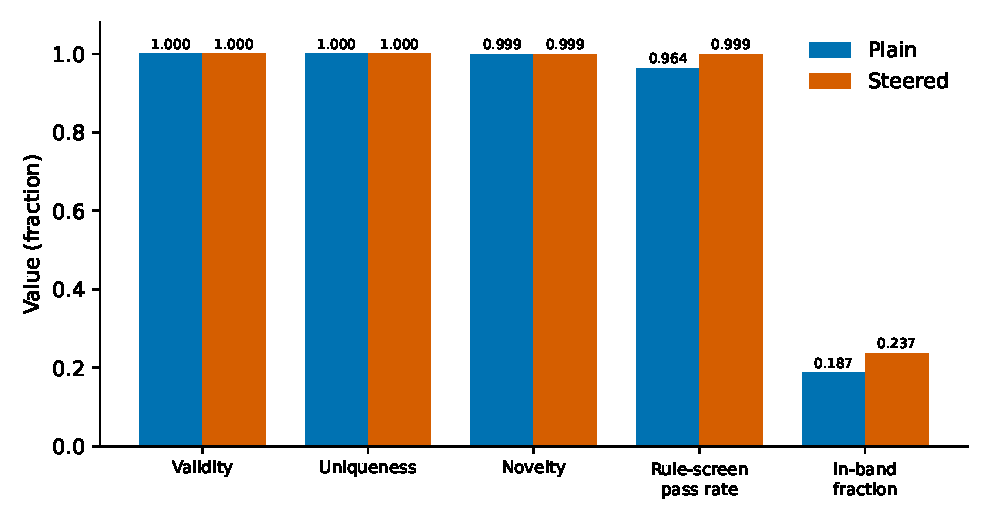
\includegraphics[width=0.85\textwidth]{figures/fig_metrics.pdf}
\caption{Per-arm evaluation metrics over 20{,}000 samples each. Validity, uniqueness and
novelty are near-identical across arms. The steered arm raises the structural-screen pass
rate and the in-band fraction.}
\label{fig:metrics}
\end{figure}

\begin{figure}[htbp]
\centering
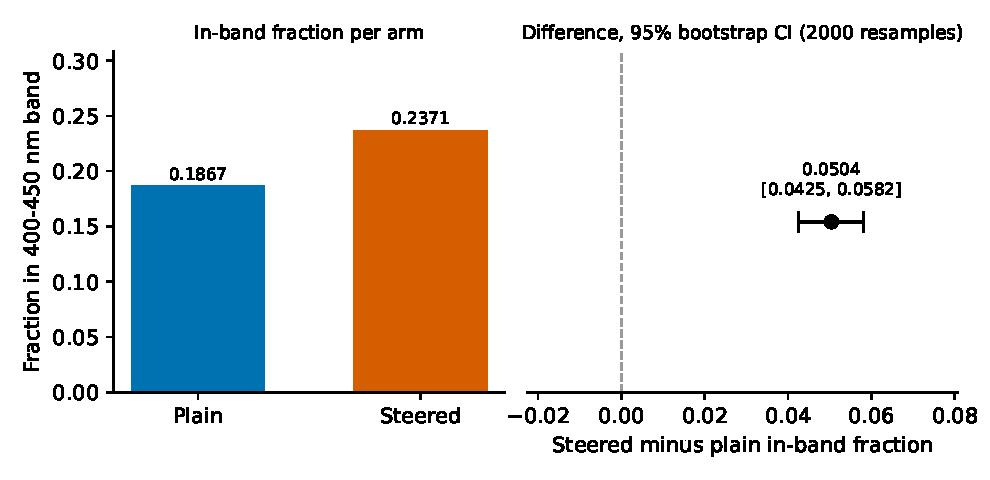
\includegraphics[width=0.95\textwidth]{figures/fig_ci.pdf}
\caption{Left: in-band fraction per arm. Right: the steered-minus-plain difference in
in-band fraction with its 95\% bootstrap confidence interval over 2{,}000 resamples. The
interval excludes zero.}
\label{fig:ci}
\end{figure}

\subsection{CPU-scale pilot}

An earlier pilot on CPU used 20 epochs over a 6{,}000-molecule ZINC subset and 3{,}000
samples per arm. There the in-band fraction was 0.244 for the plain arm and 0.257 for the
steered arm, a gap inside sampling noise at that budget. The pilot showed the pipeline ran
end to end and the direction was positive, but it could not separate the effect from
noise. The full run reported above, at 20{,}000 samples per arm on the complete corpus,
resolves a clear positive effect.

\section{Discussion}

The steering effect is real and modest. The confidence interval on the difference
excludes zero and every resample is positive, so the direction is not an artifact of a
single draw. At the same time the absolute in-band fraction stays below one quarter in the
steered arm, so most samples still fall outside the band. Prefix-token conditioning shifts
the output distribution toward the target without any per-sample guarantee, which matches
the known behaviour of soft conditioning relative to in-sampler constraint projection
\cite{cardei2025cdd, christopher2025nsd}.

The structural-screen pass rate moves almost to saturation (0.964 to 0.999), a larger
relative change than the band effect. The clean-screen token is a near-binary signal that
most training molecules already satisfy, so it is easier to push than a narrow numeric
band.

\section{Limitations}

Several limits bound these results.
\begin{itemize}
  \item The property values are surrogate predictions, not measurements. The regressor's
  held-out mean absolute error is about 24~nm, roughly half the 50~nm width of the target
  band, so individual in-band calls carry real error. The comparison is honest because
  both arms are scored by the same surrogate, but the absolute in-band fractions are not
  physical measurements.
  \item This is one run, one band and one seed. The confidence interval captures sampling
  variation at fixed weights, not variation across training seeds.
  \item Only one target band was tested. Whether the effect holds across the spectrum,
  and whether it scales with the share of in-band training examples, is untested here.
  \item The structural screen is a pattern-matching metric, not a legal or safety
  determination.
\end{itemize}

\section{Future work}

Natural extensions are multiple target bands across the spectrum, several training seeds
with a seed-level test, measured validation of a sampled subset in place of surrogate scores,
and a joint objective that steers a property target and a structural screen together and
compares soft prefix conditioning against in-sampler constraint projection on the same
task.

\section*{Data and code availability}

Code, training and evaluation scripts, and the evaluation result artifacts are public at
\url{https://github.com/cap-jmk-real/compliance-conditioned-molgen}. The experiment code is pinned at commit \texttt{0c102b6} on \texttt{main}. The numbers in this
paper are produced from the committed evaluation artifact by the figure script in
\texttt{paper/figures/}. The public datasets used are ZINC250k \cite{sterling2015zinc15}
and the UV-Vis dataset of Joung et al. \cite{joung2020uvvis}.

\section*{Conflicts of interest}

The author declares no conflict of interest.

\bibliographystyle{unsrt}
\bibliography{refs}

\end{document}
